Ogni componente ha deciso che si impegnerà al massimo delle ore, ovvero 100: quindi in totale si otterranno 700 ore. 
Il preventivo è stato calcolato sulla base del costo orario per ruolo presente nel Regolamento del Progetto Didattico.
La suddivisione dei ruoli per persona è stata fatta nel modo più equo possibile,in modo da dare a tutti i membri la possibilità di 
sperimentare ogni ruolo. \\
All’interno delle tabelle sono state utilizzate tali abbreviazioni per consentire una lettura più scorrevole:
\begin{itemize}
    \item Re :Responsabile
    \item Am: Amministratore
    \item An:Analista
    \item Pt:Progettista
    \item Pr:Programmatore
    \item Ve:Verificatore
\end{itemize}

\subsection{Primo incremento} 
{
    \subsubsection{Prospetto orario}
    {
    Il gruppo per il primo incremento si impegna a rispettare tale ruoli come riportato in tabella:
    
    \newcolumntype{L}[1]{>{\raggedright\let\newline\\\arraybackslash\hspace{1pt}}m{#1}}
      \newcolumntype{C}[1]{>{\centering\let\newline\\\arraybackslash\hspace{1pt}}m{#1}}
      \newcolumntype{R}[1]{>{\raggedleft\let\newline\\\arraybackslash\hspace{1pt}}m{#1}}

      \setlength{\freewidth}{\dimexpr\textwidth-30\tabcolsep}
      \renewcommand{\arraystretch}{1.0}
      \centering
      \setlength{\aboverulesep}{0pt}
      \setlength{\belowrulesep}{0pt}
      \begin{longtable}{C{.4\freewidth} C{.1\freewidth} C{.1\freewidth} C{.1\freewidth} C{.1\freewidth} C{.1\freewidth} C{.1\freewidth} C{.1\freewidth} C{.1\freewidth}}
      \toprule
      \rowcolor{Arancione}
      \textcolor{white}{\textbf{Componente}}&
      \textcolor{white}{\textbf{Re}}&
      \textcolor{white}{\textbf{Am}}&
      \textcolor{white}{\textbf{An}}&
      \textcolor{white}{\textbf{Pt}}&
      \textcolor{white}{\textbf{Pr}}&
      \textcolor{white}{\textbf{Ve}}&
      \textcolor{white}{\textbf{Ore}}\\
      \toprule
      \endhead

      Arena Angela & - & 4 & - & - & - & 5 & 9 \\
      \bottomrule
      Bellò Marco & 2 & 4 & - & - & - & 1 & 7 \\
      \bottomrule
      Bousapnamene & - & 3 & - & - & - & 4 & 7 \\
      \bottomrule
      Di Fant Tommaso & - & 4 & - & - & - & 4 & 8 \\
      \bottomrule
      Tossuto Matteo & - & 5 & - & - & - & 4 & 9 \\
      \bottomrule
      Volpato Marco & 3 & 2 & - & - & - & 2 & 7 \\
      \bottomrule
      Zanatta Giulio & - & 5 & - & - & - & 4 & 9 \\
      \bottomrule
      Totali & 5 & 27 & - & - & - & 24 & 56 \\
      \\
      \caption{Primo incremento - Suddivisone ore per ruolo}
      \end{longtable} 

      \begin{figure}[H]
        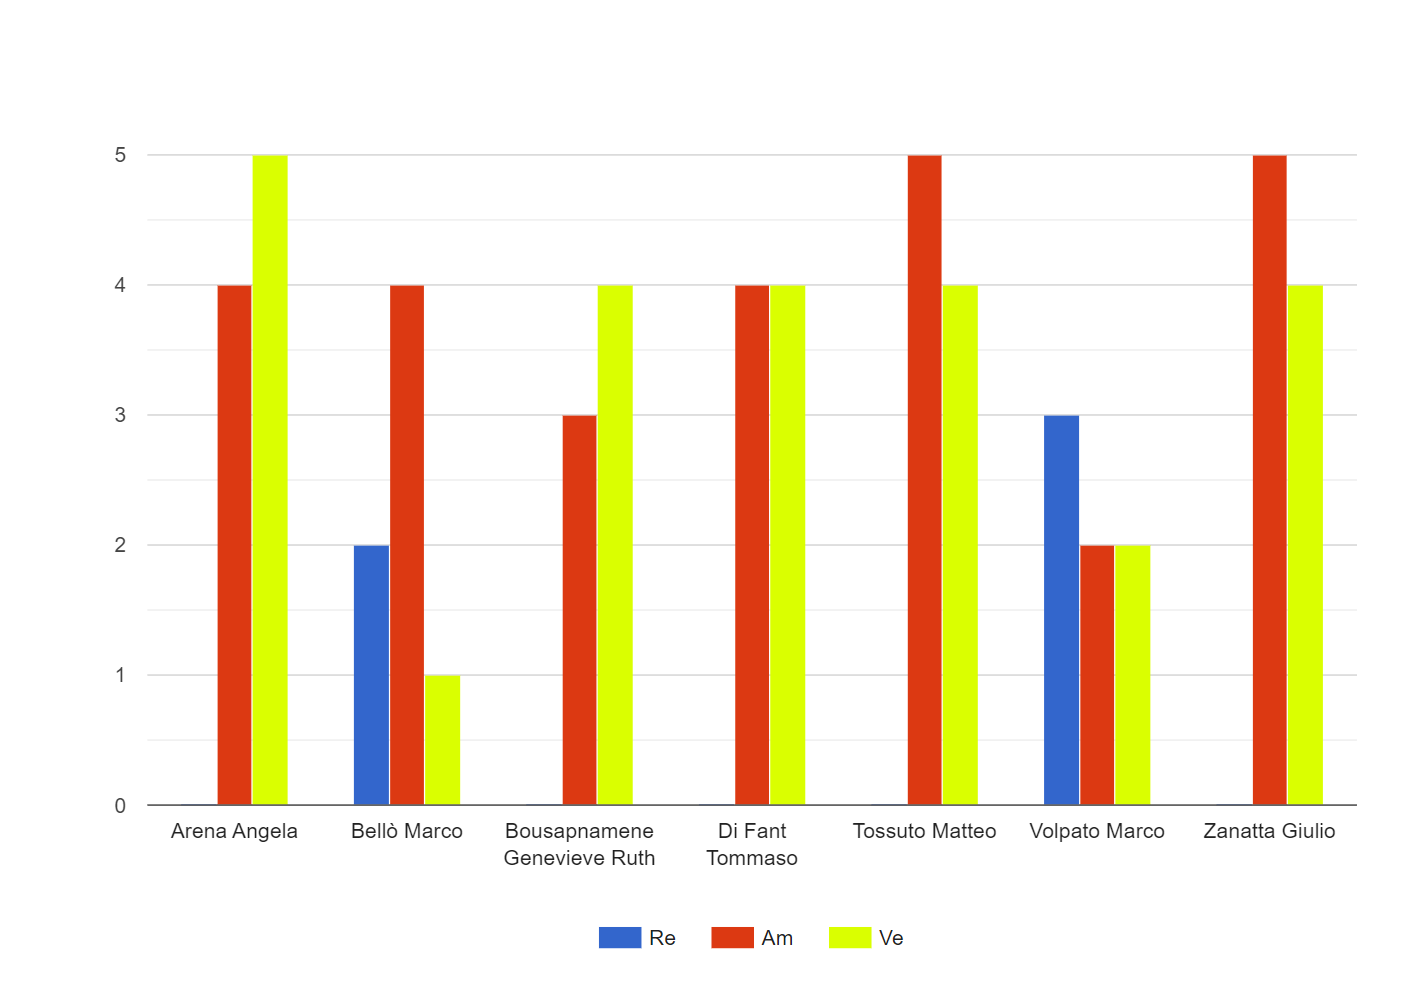
\includegraphics[width=15cm]{sezioni/Images/primo.png}
        \centering
        \\
        \caption{Primo incremento - Istogramma suddivisione ore per ruolo}
     \end{figure}
    }

    \subsubsection{Prospetto Economico}
    {
        \newcolumntype{L}[1]{>{\raggedright\let\newline\\\arraybackslash\hspace{1pt}}m{#1}}
        \newcolumntype{C}[1]{>{\centering\let\newline\\\arraybackslash\hspace{1pt}}m{#1}}
        \newcolumntype{R}[1]{>{\raggedleft\let\newline\\\arraybackslash\hspace{1pt}}m{#1}}
  
        \setlength{\freewidth}{\dimexpr\textwidth-30\tabcolsep}
        \renewcommand{\arraystretch}{1.0}
        \centering
        \setlength{\aboverulesep}{0pt}
        \setlength{\belowrulesep}{0pt}
        \begin{longtable}{C{.3\freewidth} C{.2\freewidth} C{.2\freewidth}}
          \toprule
        \rowcolor{Arancione}
        \textcolor{white}{\textbf{Ruolo}}&
        \textcolor{white}{\textbf{Ore}}&
        \textcolor{white}{\textbf{Costo}}\\
        \toprule
        \endhead
            
        Responsabile & 5 & €150\\
        \bottomrule
        Amministratore & 27 & €540\\
        \bottomrule
        Analista & - &-\\
        \bottomrule
        Progettista&-&-\\
        \bottomrule
        Programmatore&-&-\\
        \bottomrule
        Verificatore&24 & €360\\
        
        Totale&56&€1050\\
        \\
        \caption{Primo incremento - Costo per ruolo}

        \end{longtable}
        \begin{figure}[H]
          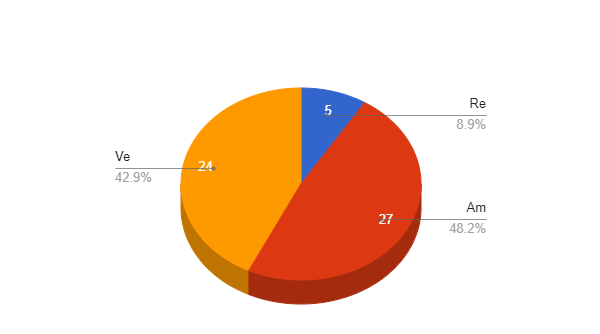
\includegraphics[width=15cm]{sezioni/Images/primoT.png}
          \centering
          \caption{Primo incremento - Grafico a torta costo per ruolo}
       \end{figure}
    }
}
  
  \subsection{Secondo incremento} 
    {
    \subsubsection{Prospetto orario}
    {
    Il gruppo per il secondo incremento si impegna a rispettare tale ruoli come riportato in tabella:
    
    \newcolumntype{L}[1]{>{\raggedright\let\newline\\\arraybackslash\hspace{1pt}}m{#1}}
      \newcolumntype{C}[1]{>{\centering\let\newline\\\arraybackslash\hspace{1pt}}m{#1}}
      \newcolumntype{R}[1]{>{\raggedleft\let\newline\\\arraybackslash\hspace{1pt}}m{#1}}

      
      \setlength{\freewidth}{\dimexpr\textwidth-30\tabcolsep}
      \renewcommand{\arraystretch}{1.0}
      \centering
      \setlength{\aboverulesep}{0pt}
      \setlength{\belowrulesep}{0pt}
      \begin{longtable}{C{.4\freewidth} C{.1\freewidth} C{.1\freewidth} C{.1\freewidth} C{.1\freewidth} C{.1\freewidth} C{.1\freewidth} C{.1\freewidth} C{.1\freewidth}}
      \toprule
      \rowcolor{Arancione}
      \textcolor{white}{\textbf{Componente}}&
      \textcolor{white}{\textbf{Re}}&
      \textcolor{white}{\textbf{Am}}&
      \textcolor{white}{\textbf{An}}&
      \textcolor{white}{\textbf{Pt}}&
      \textcolor{white}{\textbf{Pr}}&
      \textcolor{white}{\textbf{Ve}}&
      \textcolor{white}{\textbf{Ore}}\\
      \toprule
      \endhead

      Arena Angela & - & - & 7  & - & - & 4 & 11 \\
      \bottomrule
      Bellò Marco & - & - & 8 & - & - & 4 & 12 \\
      \bottomrule
      Bousapnamene & 5 & - & 2 & - & - & 4 & 11 \\
      \bottomrule
      Di Fant Tommaso & - & - & 6 & - & - & 4 & 10 \\
      \bottomrule
      Tossuto Matteo & - & - & 9 & - & - & 1 & 10 \\
      \bottomrule
      Volpato Marco & - & - & 9 & - & - & 2 & 11 \\
      \bottomrule
      Zanatta Giulio & - & - & 8 & - & - & 4 & 12 \\
      \bottomrule
      Totali & 5 & - & 49 & - & - & 23 & 77 \\
      \\
      \caption{Secondo incremento - Suddivisone ore per ruolo}

      \end{longtable} 
      \begin{figure}[H]
        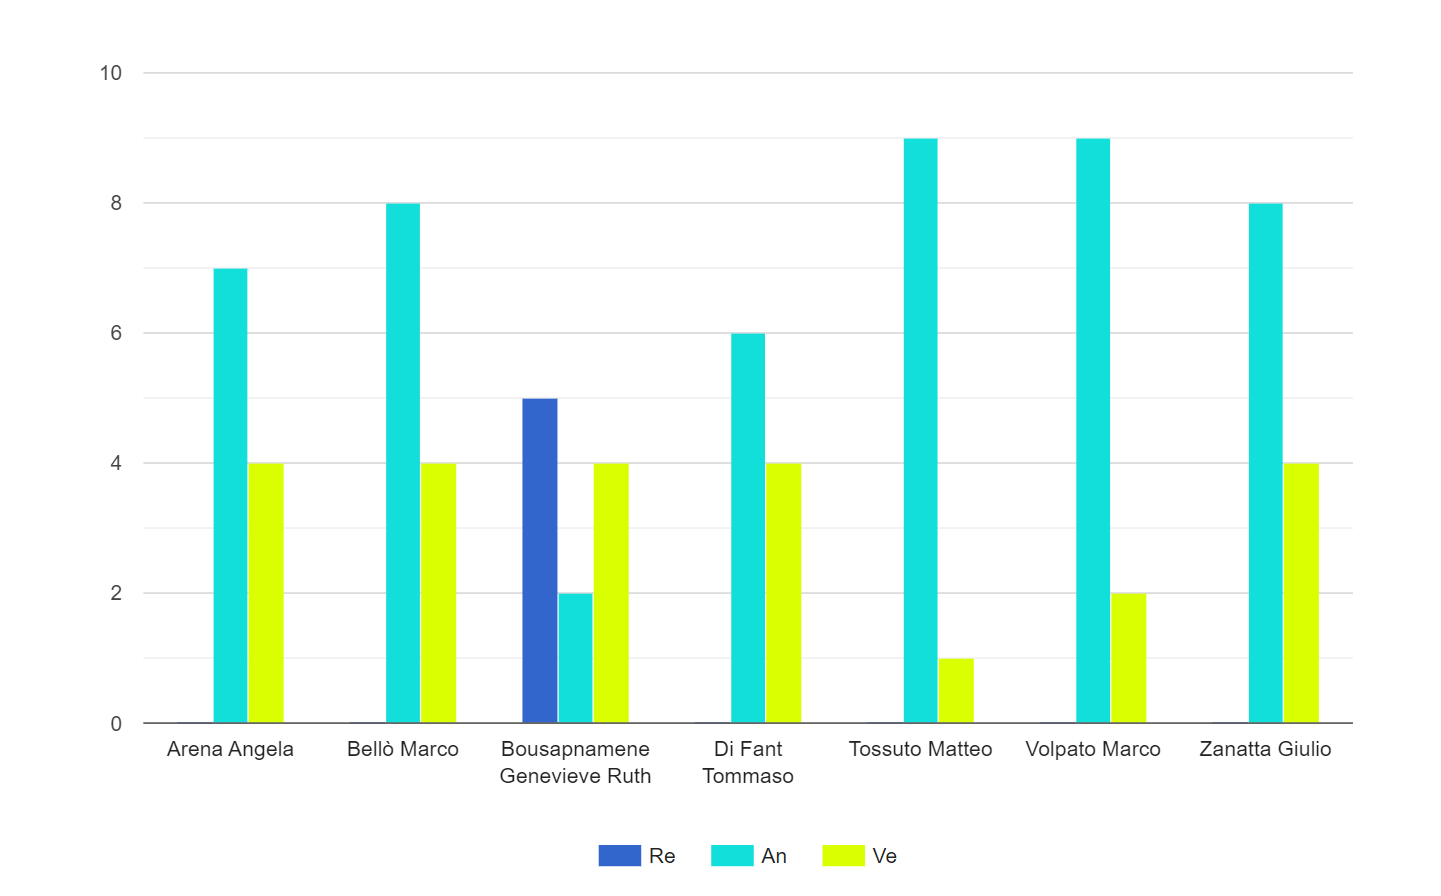
\includegraphics[width=15cm]{sezioni/Images/secondo.png}
        \centering
        \caption{Secondo incremento - Istogramma suddivisione ore per ruolo}
     \end{figure}
      
    }
    

    \subsubsection{Prospetto Economico}
    {
        \newcolumntype{L}[1]{>{\raggedright\let\newline\\\arraybackslash\hspace{1pt}}m{#1}}
        \newcolumntype{C}[1]{>{\centering\let\newline\\\arraybackslash\hspace{1pt}}m{#1}}
        \newcolumntype{R}[1]{>{\raggedleft\let\newline\\\arraybackslash\hspace{1pt}}m{#1}}
  
        \setlength{\freewidth}{\dimexpr\textwidth-30\tabcolsep}
        \renewcommand{\arraystretch}{1.0}
        \centering
        \setlength{\aboverulesep}{0pt}
        \setlength{\belowrulesep}{0pt}
        \begin{longtable}{C{.4\freewidth} C{.2\freewidth} C{.2\freewidth} C{.2\freewidth} C{.2\freewidth} C{.2\freewidth} C{.2\freewidth} C{.2\freewidth} C{.2\freewidth}}
          \toprule
        \rowcolor{Arancione}
        \textcolor{white}{\textbf{Ruolo}}&
        \textcolor{white}{\textbf{Ore}}&
        \textcolor{white}{\textbf{Costo}}\\
        \toprule
        \endhead
            
        Responsabile  & 5 & €150\\
        \bottomrule
        Amministratore  & -&  \\
        \bottomrule
        Analista &49 & €1225\\
        \bottomrule
        Progettista &- &\\
        \bottomrule
        Programmatore &- & \\
        \bottomrule
        Verificatore &23 &€345\\
        \bottomrule
        Totale&77&€1720\\
        \\
        \caption{Secondo incremento - Costo per ruolo}

        \end{longtable}
        \begin{figure}[H]
          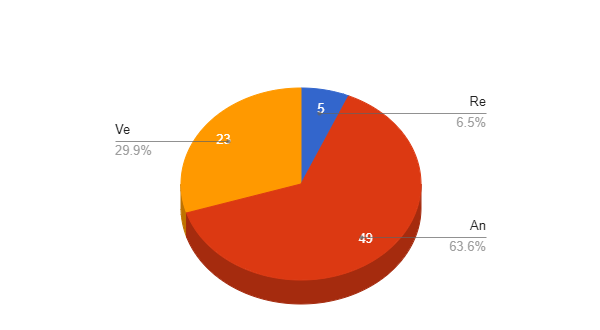
\includegraphics[width=15cm]{sezioni/Images/secondoT.png}
          \centering
          \caption{Secondo incremento - Grafico a torta costo per ruolo}
       \end{figure}
    }
    }

    \subsection{Terzo incremento} 
    {
    \subsubsection{Prospetto orario}
    {
    Il gruppo per il terzo incremento si impegna a rispettare tale ruoli come riportato in tabella:
    
    \newcolumntype{L}[1]{>{\raggedright\let\newline\\\arraybackslash\hspace{1pt}}m{#1}}
      \newcolumntype{C}[1]{>{\centering\let\newline\\\arraybackslash\hspace{1pt}}m{#1}}
      \newcolumntype{R}[1]{>{\raggedleft\let\newline\\\arraybackslash\hspace{1pt}}m{#1}}

      
      \setlength{\freewidth}{\dimexpr\textwidth-30\tabcolsep}
      \renewcommand{\arraystretch}{1.0}
      \centering
      \setlength{\aboverulesep}{0pt}
      \setlength{\belowrulesep}{0pt}
      \begin{longtable}{C{.4\freewidth} C{.1\freewidth} C{.1\freewidth} C{.1\freewidth} C{.1\freewidth} C{.1\freewidth} C{.1\freewidth} C{.1\freewidth} C{.1\freewidth}}
      \toprule
      \rowcolor{Arancione}
      \textcolor{white}{\textbf{Componente}}&
      \textcolor{white}{\textbf{Re}}&
      \textcolor{white}{\textbf{Am}}&
      \textcolor{white}{\textbf{An}}&
      \textcolor{white}{\textbf{Pt}}&
      \textcolor{white}{\textbf{Pr}}&
      \textcolor{white}{\textbf{Ve}}&
      \textcolor{white}{\textbf{Ore}}\\
      \toprule
      \endhead

      Arena Angela & 2 & - & 4  & 2 & 2 & 4 & 14 \\
      \bottomrule
      Bellò Marco & - & 1 & 1 & 5 & 7 & - & 14 \\
      \bottomrule
      Bousapnamene & - & 2 & - & 6 & 4 & 2 & 14 \\
      \bottomrule
      Di Fant Tommaso & - & - & - & 7 & 8 & 1 & 16 \\
      \bottomrule
      Tossuto Matteo & - & - & 4 & 3 & 7 & - & 14 \\
      \bottomrule
      Volpato Marco & - & - & - & 3 & 9 & 2 & 14 \\
      \bottomrule
      Zanatta Giulio & 3 & 2 & - & - & 5 & 3 & 13 \\
      \bottomrule
      Totali & 5 & 5 & 9 & 26 & 42 & 12 & 99 \\
      \\
      \caption{Terzo incremento - Suddivisone ore per ruolo}

      \end{longtable} 

      \begin{figure}[H]
        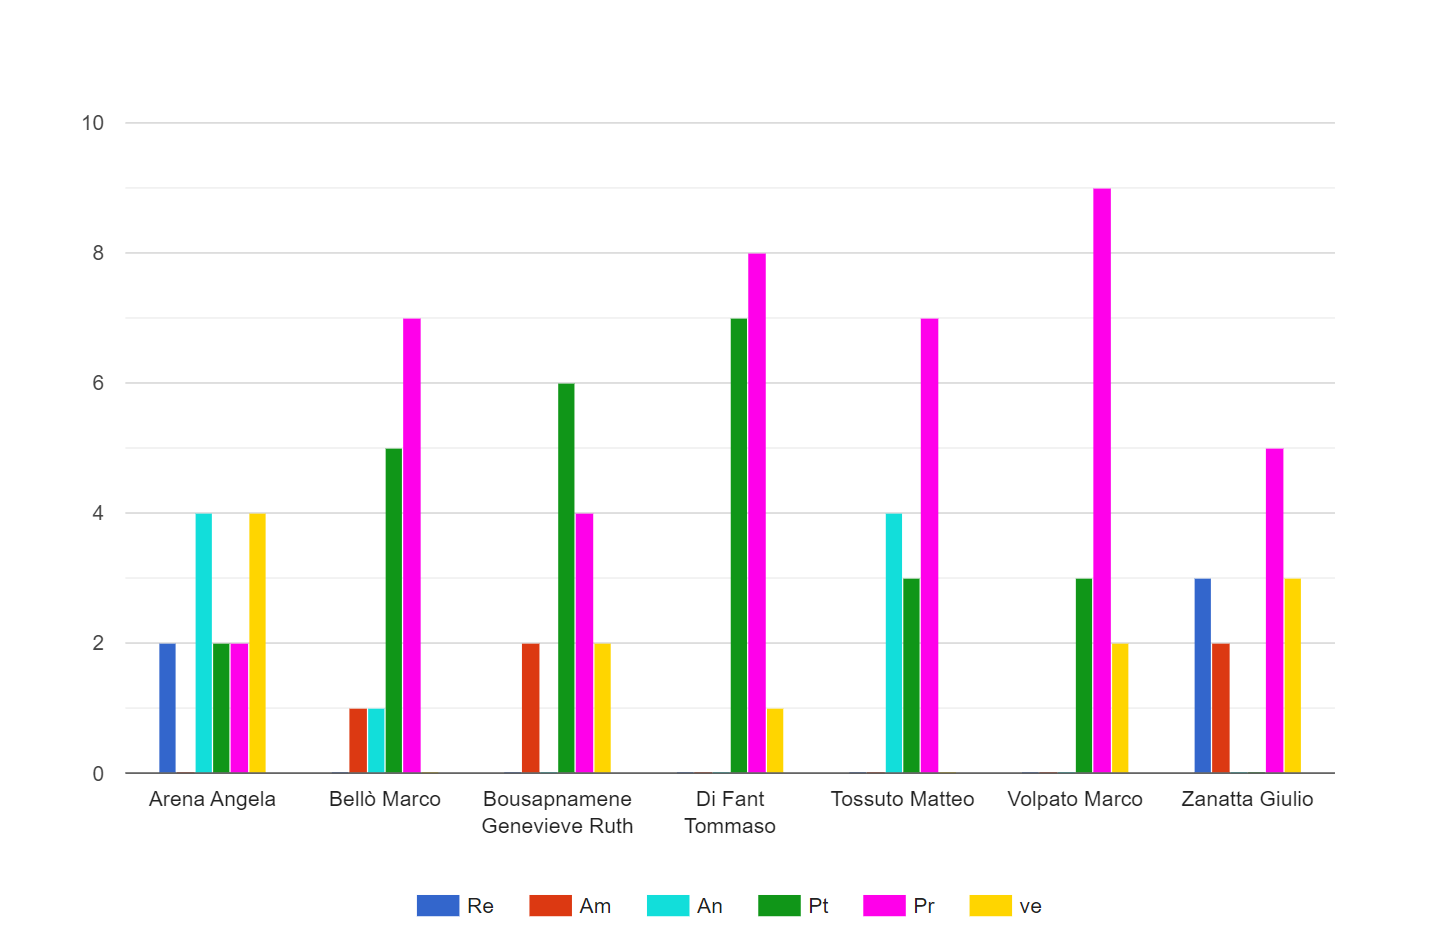
\includegraphics[width=15cm]{sezioni/Images/terzo.png}
        \centering
        \caption{Terzo incremento - Istogramma suddivisione ore per ruolo}
     \end{figure}
    }

    \subsubsection{Prospetto Economico}
    {
        \newcolumntype{L}[1]{>{\raggedright\let\newline\\\arraybackslash\hspace{1pt}}m{#1}}
        \newcolumntype{C}[1]{>{\centering\let\newline\\\arraybackslash\hspace{1pt}}m{#1}}
        \newcolumntype{R}[1]{>{\raggedleft\let\newline\\\arraybackslash\hspace{1pt}}m{#1}}
  
        \setlength{\freewidth}{\dimexpr\textwidth-30\tabcolsep}
        \renewcommand{\arraystretch}{1.0}
        \centering
        \setlength{\aboverulesep}{0pt}
        \setlength{\belowrulesep}{0pt}
        \begin{longtable}{C{.4\freewidth} C{.2\freewidth} C{.2\freewidth} C{.2\freewidth} C{.2\freewidth} C{.2\freewidth} C{.2\freewidth} C{.2\freewidth} C{.2\freewidth}}
          \toprule
        \rowcolor{Arancione}
        \textcolor{white}{\textbf{Ruolo}}&
        \textcolor{white}{\textbf{Ore}}&
        \textcolor{white}{\textbf{Costo}}\\
        \toprule
        \endhead
            
        Responsabile  & 5 & €150\\
        Amministratore  & 5 & €100 \\
        Analista &9 & €225\\
        Progettista &26 & €650\\
        Programmatore &42 & €630\\
        Verificatore &12 & €180\\
        Totale&99&€1935\\
        \\
        \caption{Terzo incremento - Costo per ruolo}

        \end{longtable}
        \begin{figure}[H]
          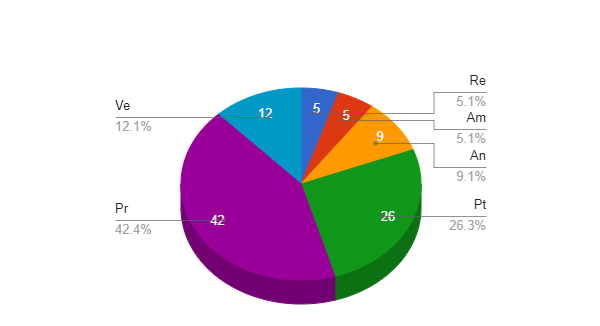
\includegraphics[width=15cm]{sezioni/Images/terzoT.png}
          \centering
          \caption{Terzo incremento - Grafico a torta costo per ruolo}
       \end{figure}
    }
    }

    \subsection{Quarto incremento} 
    {
    \subsubsection{Prospetto orario}
    {
    Il gruppo per il quarto incremento si impegna a rispettare tale ruoli come riportato in tabella:
    
    \newcolumntype{L}[1]{>{\raggedright\let\newline\\\arraybackslash\hspace{1pt}}m{#1}}
      \newcolumntype{C}[1]{>{\centering\let\newline\\\arraybackslash\hspace{1pt}}m{#1}}
      \newcolumntype{R}[1]{>{\raggedleft\let\newline\\\arraybackslash\hspace{1pt}}m{#1}}

      
      \setlength{\freewidth}{\dimexpr\textwidth-30\tabcolsep}
      \renewcommand{\arraystretch}{1.0}
      \centering
      \setlength{\aboverulesep}{0pt}
      \setlength{\belowrulesep}{0pt}
      \begin{longtable}{C{.4\freewidth} C{.1\freewidth} C{.1\freewidth} C{.1\freewidth} C{.1\freewidth} C{.1\freewidth} C{.1\freewidth} C{.1\freewidth} C{.1\freewidth}}
      \toprule
      \rowcolor{Arancione}
      \textcolor{white}{\textbf{Componente}}&
      \textcolor{white}{\textbf{Re}}&
      \textcolor{white}{\textbf{Am}}&
      \textcolor{white}{\textbf{An}}&
      \textcolor{white}{\textbf{Pt}}&
      \textcolor{white}{\textbf{Pr}}&
      \textcolor{white}{\textbf{Ve}}&
      \textcolor{white}{\textbf{Ore}}\\
      \toprule
      \endhead

      Arena Angela & - & 2 & -  & 10 & - & 2 & 14 \\
      \bottomrule
      Bellò Marco & - & 2 & - & 9 & - & 2 & 13 \\
      \bottomrule
      Bousapnamene & - & 1 & - & 10 & - & 2 & 13 \\
      \bottomrule
      Di Fant Tommaso & 3 & - & - & 8 & - & 4 & 13 \\
      \bottomrule
      Tossuto Matteo & 2 & - & - & 8 & - & 3 & 15 \\
      \bottomrule
      Volpato Marco & - & 1 & - & 12 & - & 2 & 16 \\
      \bottomrule
      Zanatta Giulio & - & 1 & - & 11 & - & 3 & 15 \\
      \bottomrule
      Totali & 5 & 7 & - & 68 & - & 18 & 101 \\
      \\
      \caption{Quarto incremento - Suddivisione ore per ruolo} 

      \end{longtable} 

      \begin{figure}[H]
        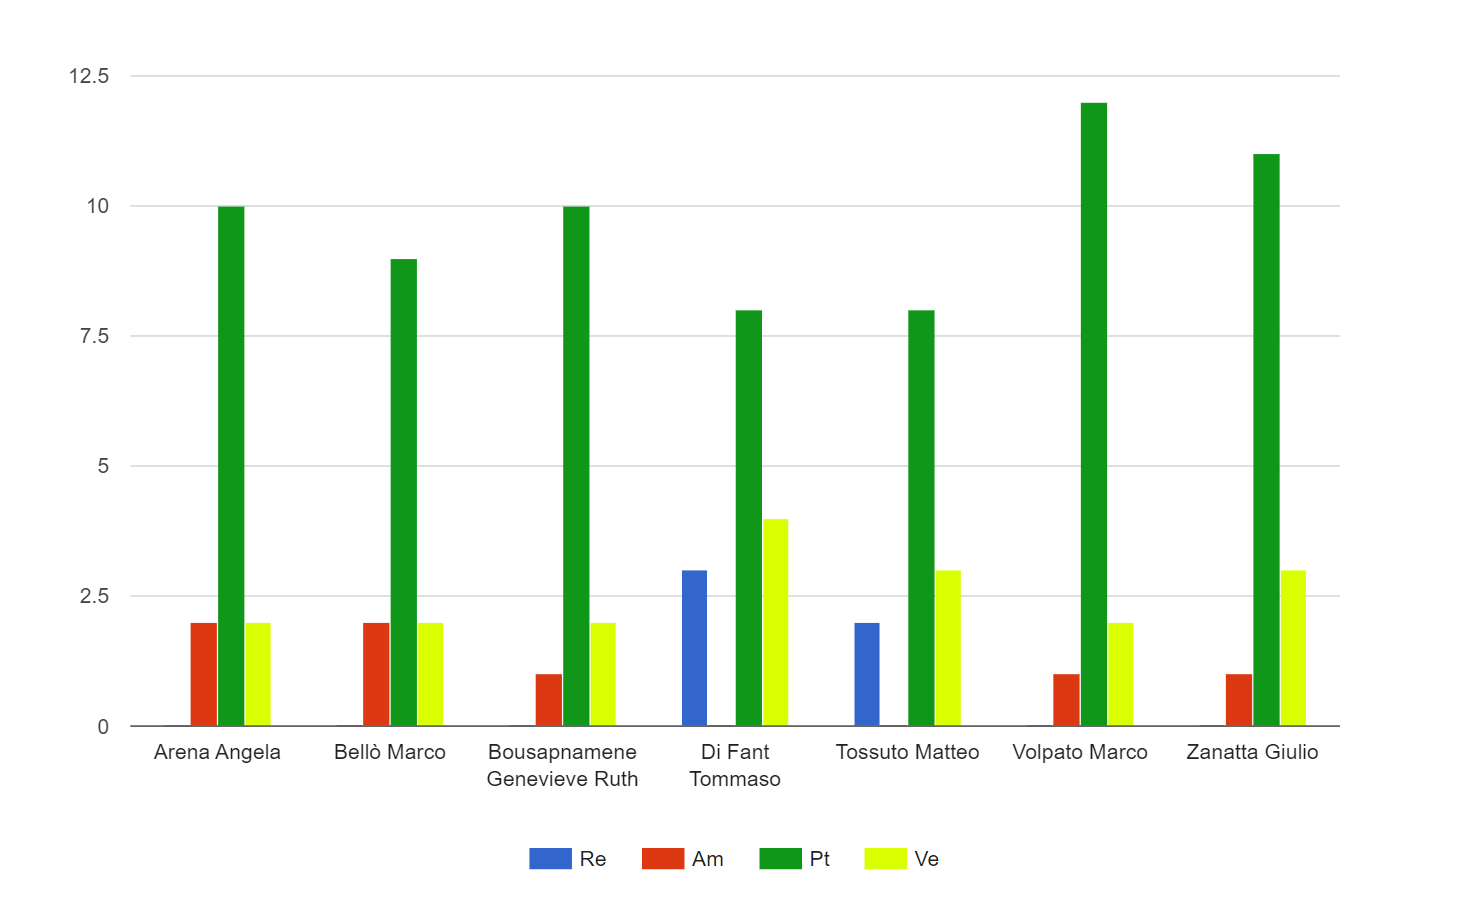
\includegraphics[width=15cm]{sezioni/Images/quarto.png}
        \centering
        \caption{Quarto incremento - Istogramma suddivisione ore per ruolo}
     \end{figure}
    }

    \subsubsection{Prospetto Economico}
    {
        \newcolumntype{L}[1]{>{\raggedright\let\newline\\\arraybackslash\hspace{1pt}}m{#1}}
        \newcolumntype{C}[1]{>{\centering\let\newline\\\arraybackslash\hspace{1pt}}m{#1}}
        \newcolumntype{R}[1]{>{\raggedleft\let\newline\\\arraybackslash\hspace{1pt}}m{#1}}
  
        \setlength{\freewidth}{\dimexpr\textwidth-30\tabcolsep}
        \renewcommand{\arraystretch}{1.0}
        \centering
        \setlength{\aboverulesep}{0pt}
        \setlength{\belowrulesep}{0pt}
        \begin{longtable}{C{.4\freewidth} C{.2\freewidth} C{.2\freewidth} C{.2\freewidth} C{.2\freewidth} C{.2\freewidth} C{.2\freewidth} C{.2\freewidth} C{.2\freewidth}}
          \toprule
        \rowcolor{Arancione}
        \textcolor{white}{\textbf{Ruolo}}&
        \textcolor{white}{\textbf{Ore}}&
        \textcolor{white}{\textbf{Costo}}\\
        \toprule
        \endhead
            
        Responsabile  & 5 & €150\\
        Amministratore  & 7& €140 \\
        Analista &- & -\\
        Progettista &68 &€1700\\
        Programmatore &- & -\\
        Verificatore &18 &€270\\
        Totale&101&€2260\\
        \\
        \caption{Quarto incremento - Costo per ruolo}

        \end{longtable}
        \begin{figure}[H]
          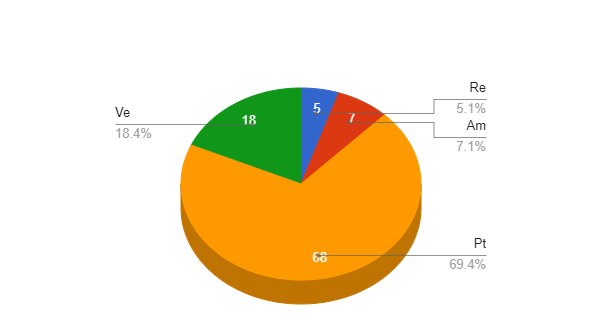
\includegraphics[width=15cm]{sezioni/Images/quartoT.png}
          \centering
          \caption{Quarto incremento - Grafico a torta costo per ruolo}
       \end{figure}
    }
    }

    \subsection{Quinto incremento} 
    {
    \subsubsection{Prospetto orario}
    {
    Il gruppo per il quinto incremento si impegna a rispettare tale ruoli come riportato in tabella:
    
    \newcolumntype{L}[1]{>{\raggedright\let\newline\\\arraybackslash\hspace{1pt}}m{#1}}
      \newcolumntype{C}[1]{>{\centering\let\newline\\\arraybackslash\hspace{1pt}}m{#1}}
      \newcolumntype{R}[1]{>{\raggedleft\let\newline\\\arraybackslash\hspace{1pt}}m{#1}}

      
      \setlength{\freewidth}{\dimexpr\textwidth-30\tabcolsep}
      \renewcommand{\arraystretch}{1.0}
      \centering
      \setlength{\aboverulesep}{0pt}
      \setlength{\belowrulesep}{0pt}
      \begin{longtable}{C{.4\freewidth} C{.1\freewidth} C{.1\freewidth} C{.1\freewidth} C{.1\freewidth} C{.1\freewidth} C{.1\freewidth} C{.1\freewidth} C{.1\freewidth}}
      \toprule
      \rowcolor{Arancione}
      \textcolor{white}{\textbf{Componente}}&
      \textcolor{white}{\textbf{Re}}&
      \textcolor{white}{\textbf{Am}}&
      \textcolor{white}{\textbf{An}}&
      \textcolor{white}{\textbf{Pt}}&
      \textcolor{white}{\textbf{Pr}}&
      \textcolor{white}{\textbf{Ve}}&
      \textcolor{white}{\textbf{Ore}}\\
      \toprule
      \endhead

      Arena Angela & - & 3 & -  & 6 & 10 & 2 & 21 \\
      \bottomrule
      Bellò Marco & - & - & - & 6 & 10 & 3 & 19 \\
      \bottomrule
      Bousapnamene & 2 & - & - & 5 & 10 & 4 & 21 \\
      \bottomrule
      Di Fant Tommaso & - & 1 & - & 6 & 12 & 3 & 22 \\
      \bottomrule
      Tossuto Matteo & - & 1 & - & 8 & 12 & 1 & 22 \\
      \bottomrule
      Volpato Marco & 3 & - & - & 4 & 10 & 5 & 22 \\
      \bottomrule
      Zanatta Giulio & - & 2 & - & 6 & 11 & 3 & 21 \\
      \bottomrule
      Totali & 5 & 7 & - & 41 & 75 & 21 & 148 \\
      \\
      \caption{Quinto incremento - Suddivisione ore per ruolo}
      \end{longtable} 

      \begin{figure}[H]
        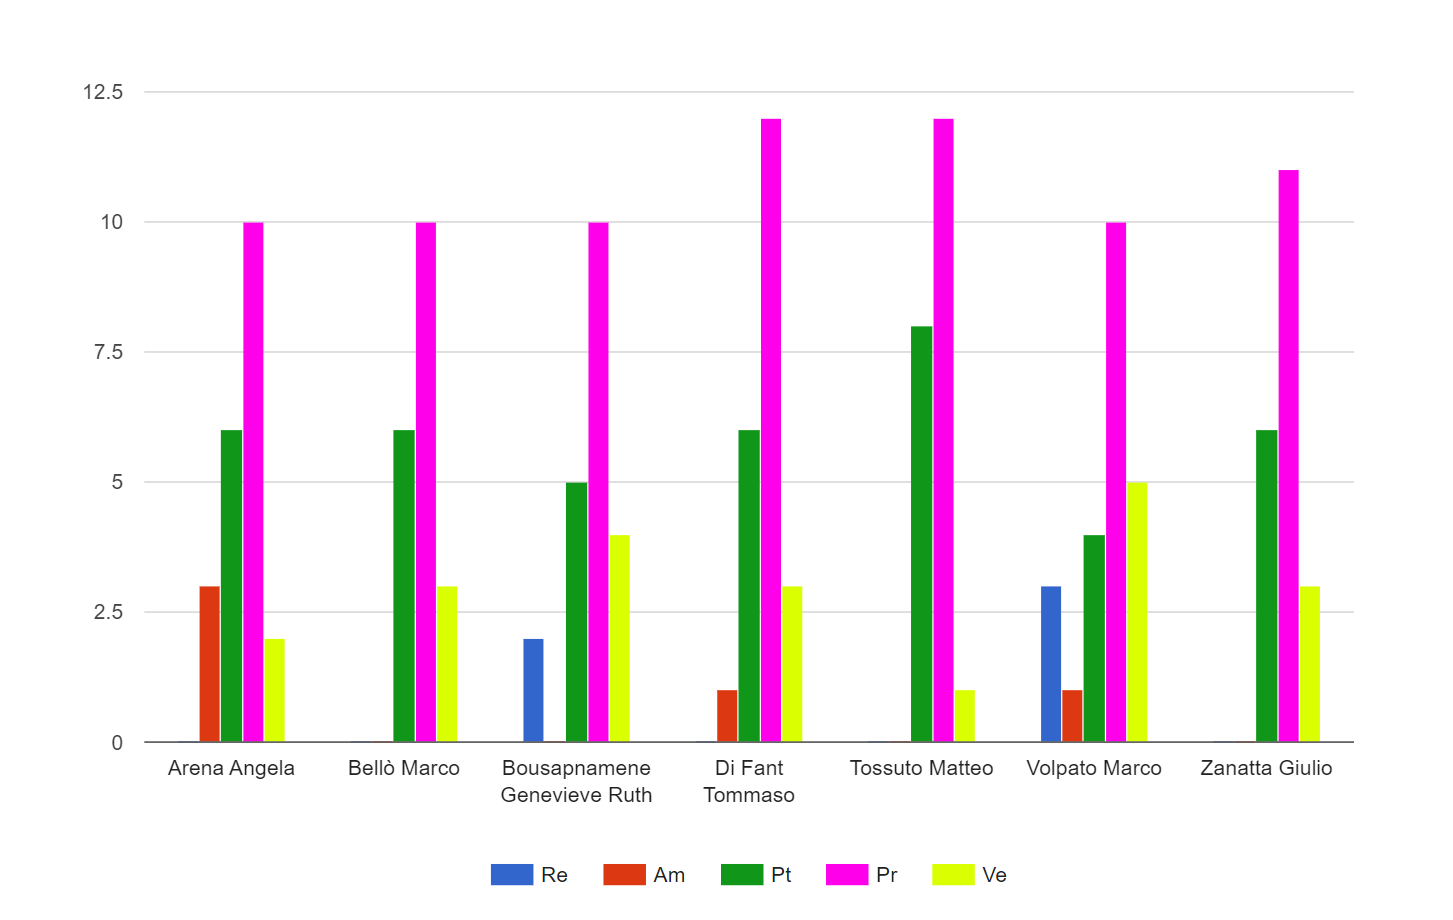
\includegraphics[width=15cm]{sezioni/Images/quinto.png}
        \centering
        \caption{Quinto incremento - Istogramma suddivisone ore per ruolo}
     \end{figure}
    }

    \subsubsection{Prospetto Economico}
    {
        \newcolumntype{L}[1]{>{\raggedright\let\newline\\\arraybackslash\hspace{1pt}}m{#1}}
        \newcolumntype{C}[1]{>{\centering\let\newline\\\arraybackslash\hspace{1pt}}m{#1}}
        \newcolumntype{R}[1]{>{\raggedleft\let\newline\\\arraybackslash\hspace{1pt}}m{#1}}
  
        \setlength{\freewidth}{\dimexpr\textwidth-30\tabcolsep}
        \renewcommand{\arraystretch}{1.0}
        \centering
        \setlength{\aboverulesep}{0pt}
        \setlength{\belowrulesep}{0pt}
        \begin{longtable}{C{.4\freewidth} C{.2\freewidth} C{.2\freewidth} C{.2\freewidth} C{.2\freewidth} C{.2\freewidth} C{.2\freewidth} C{.2\freewidth} C{.2\freewidth}}
          \toprule
        \rowcolor{Arancione}
        \textcolor{white}{\textbf{Ruolo}}&
        \textcolor{white}{\textbf{Ore}}&
        \textcolor{white}{\textbf{Costo}}\\
        \toprule
        \endhead
            
        Responsabile  & 5 & €150\\
        Amministratore  & 7 & €140 \\
        Analista &- & -\\
        Progettista &41 &€1025\\
        Programmatore &75 & €1125\\
        Verificatore &21 &€315\\
        Totale&148&€2755\\
        \\
        \caption{Quinto incremento - Costo per ruolo}

        \end{longtable}
        \begin{figure}[H]
          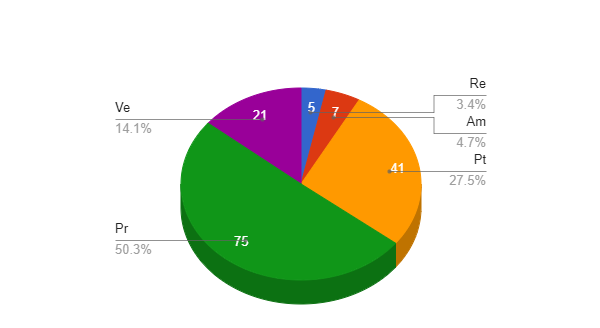
\includegraphics[width=15cm]{sezioni/Images/quintoT.png}
          \centering
          \caption{Quinto incremento - Grafico a torta costo per ruolo}
       \end{figure}
    }
    }

    \subsection{Sesto incremento} 
    {
    \subsubsection{Prospetto orario}
    {
    Il gruppo per il sesto incremento si impegna a rispettare tale ruoli come riportato in tabella:
    
    \newcolumntype{L}[1]{>{\raggedright\let\newline\\\arraybackslash\hspace{1pt}}m{#1}}
      \newcolumntype{C}[1]{>{\centering\let\newline\\\arraybackslash\hspace{1pt}}m{#1}}
      \newcolumntype{R}[1]{>{\raggedleft\let\newline\\\arraybackslash\hspace{1pt}}m{#1}}

      
      \setlength{\freewidth}{\dimexpr\textwidth-30\tabcolsep}
      \renewcommand{\arraystretch}{1.0}
      \centering
      \setlength{\aboverulesep}{0pt}
      \setlength{\belowrulesep}{0pt}
      \begin{longtable}{C{.4\freewidth} C{.1\freewidth} C{.1\freewidth} C{.1\freewidth} C{.1\freewidth} C{.1\freewidth} C{.1\freewidth} C{.1\freewidth} C{.1\freewidth}}
      \toprule
      \rowcolor{Arancione}
      \textcolor{white}{\textbf{Componente}}&
      \textcolor{white}{\textbf{Re}}&
      \textcolor{white}{\textbf{Am}}&
      \textcolor{white}{\textbf{An}}&
      \textcolor{white}{\textbf{Pt}}&
      \textcolor{white}{\textbf{Pr}}&
      \textcolor{white}{\textbf{Ve}}&
      \textcolor{white}{\textbf{Ore}}\\
      \toprule
      \endhead

      Arena Angela & 4 & - & -  & 1 & 3 & 4 & 12 \\
      \bottomrule
      Bellò Marco & 3 & - & - & 2 & 6 & 2 & 13 \\
      \bottomrule
      Bousapnamene & - & - & - & 3 & 7 & 2 & 13 \\
      \bottomrule
      Di Fant Tommaso & - & - & - & 1 & 8 & 4 & 13 \\
      \bottomrule
      Tossuto Matteo & - & - & - & 3 & 8 & 1 & 12 \\
      \bottomrule
      Volpato Marco & - & - & - & 2 & 9 & 3 & 14 \\
      \bottomrule
      Zanatta Giulio & - & - & - & 2 & 8 & 2 & 12 \\
      \bottomrule
      Totali & 7 & - & - & 14 & 49 & 18 & 89 \\
      \\
      \caption{Sesto incremento - Suddivisone ore per ruolo}

      \end{longtable} 

      \begin{figure}[H]
        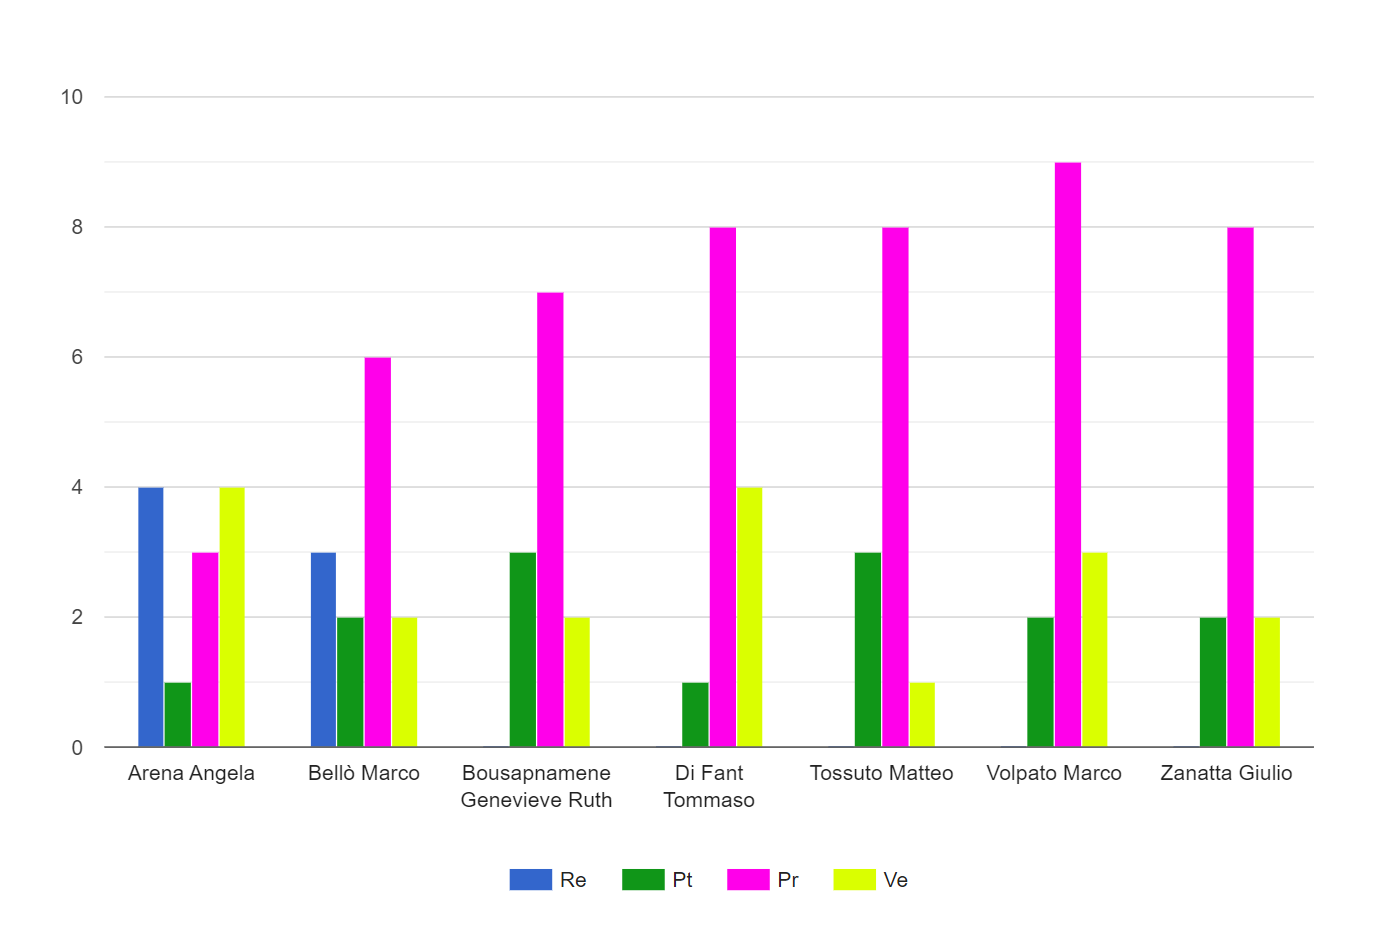
\includegraphics[width=15cm]{sezioni/Images/sesto.png}
        \centering
        \caption{Sesto incremento - Istogramma suddivisone ore per ruolo}
     \end{figure}
    }

    \subsubsection{Prospetto Economico}
    {
        \newcolumntype{L}[1]{>{\raggedright\let\newline\\\arraybackslash\hspace{1pt}}m{#1}}
        \newcolumntype{C}[1]{>{\centering\let\newline\\\arraybackslash\hspace{1pt}}m{#1}}
        \newcolumntype{R}[1]{>{\raggedleft\let\newline\\\arraybackslash\hspace{1pt}}m{#1}}
  
        \setlength{\freewidth}{\dimexpr\textwidth-30\tabcolsep}
        \renewcommand{\arraystretch}{1.0}
        \centering
        \setlength{\aboverulesep}{0pt}
        \setlength{\belowrulesep}{0pt}
        \begin{longtable}{C{.4\freewidth} C{.2\freewidth} C{.2\freewidth} C{.2\freewidth} C{.2\freewidth} C{.2\freewidth} C{.2\freewidth} C{.2\freewidth} C{.2\freewidth}}
          \toprule
        \rowcolor{Arancione}
        \textcolor{white}{\textbf{Ruolo}}&
        \textcolor{white}{\textbf{Ore}}&
        \textcolor{white}{\textbf{Costo}}\\
        \toprule
        \endhead
            
        Responsabile  & 7 & €210\\
        Amministratore  & - & - \\
        Analista &- & -\\
        Progettista &14 &€350\\
        Programmatore &49 & €735\\
        Verificatore &18 &€270\\
        Totale&89&€1565\\
        \caption{Sesto incremento - Costo per ruolo}

        \end{longtable}
        \begin{figure}[H]
          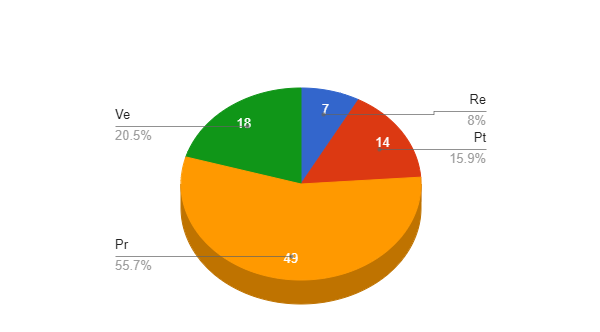
\includegraphics[width=15cm]{sezioni/Images/sestoT.png}
          \centering
          \caption{Sesto incremento - Grafico a torta costo per ruolo}
       \end{figure}
    }
    }

    \subsection{Settimo incremento} 
    {
    \subsubsection{Prospetto orario}
    {
    Il gruppo per il settimo incremento si impegna a rispettare tale ruoli come riportato in tabella:
    
    \newcolumntype{L}[1]{>{\raggedright\let\newline\\\arraybackslash\hspace{1pt}}m{#1}}
      \newcolumntype{C}[1]{>{\centering\let\newline\\\arraybackslash\hspace{1pt}}m{#1}}
      \newcolumntype{R}[1]{>{\raggedleft\let\newline\\\arraybackslash\hspace{1pt}}m{#1}}

      
      \setlength{\freewidth}{\dimexpr\textwidth-30\tabcolsep}
      \renewcommand{\arraystretch}{1.0}
      \centering
      \setlength{\aboverulesep}{0pt}
      \setlength{\belowrulesep}{0pt}
      \begin{longtable}{C{.4\freewidth} C{.1\freewidth} C{.1\freewidth} C{.1\freewidth} C{.1\freewidth} C{.1\freewidth} C{.1\freewidth} C{.1\freewidth} C{.1\freewidth}}
      \toprule
      \rowcolor{Arancione}
      \textcolor{white}{\textbf{Componente}}&
      \textcolor{white}{\textbf{Re}}&
      \textcolor{white}{\textbf{Am}}&
      \textcolor{white}{\textbf{An}}&
      \textcolor{white}{\textbf{Pt}}&
      \textcolor{white}{\textbf{Pr}}&
      \textcolor{white}{\textbf{Ve}}&
      \textcolor{white}{\textbf{Ore}}\\
      \toprule
      \endhead

      Arena Angela & - & 1 & -  & 2 & 3 & 4 & 13 \\
      \bottomrule
      Bellò Marco & - & 2 & - & 2 & 3 & 5 & 12 \\
      \bottomrule
      Bousapnamene & - & 2 & - & 1 & 4 & 4 & 11 \\
      \bottomrule
      Di Fant Tommaso & 3 & 2 & - & 3 & 2 & 2 & 12 \\
      \bottomrule
      Tossuto Matteo & 5 & 1 & - & 1 & 1 & 3 & 12 \\
      \bottomrule
      Volpato Marco & - & - & - & 5 & 3 & 4 & 12 \\
      \bottomrule
      Zanatta Giulio & - & 2 & - & 3 & 3 & 5 & 12 \\
      \bottomrule
      Totali & 8 & 10 & - & 18 & 20 & 27 & 84 \\
      \\
      \caption{Settimo incremento - Suddivisone ore per ruolo}

      \end{longtable} 

      \begin{figure}[H]
        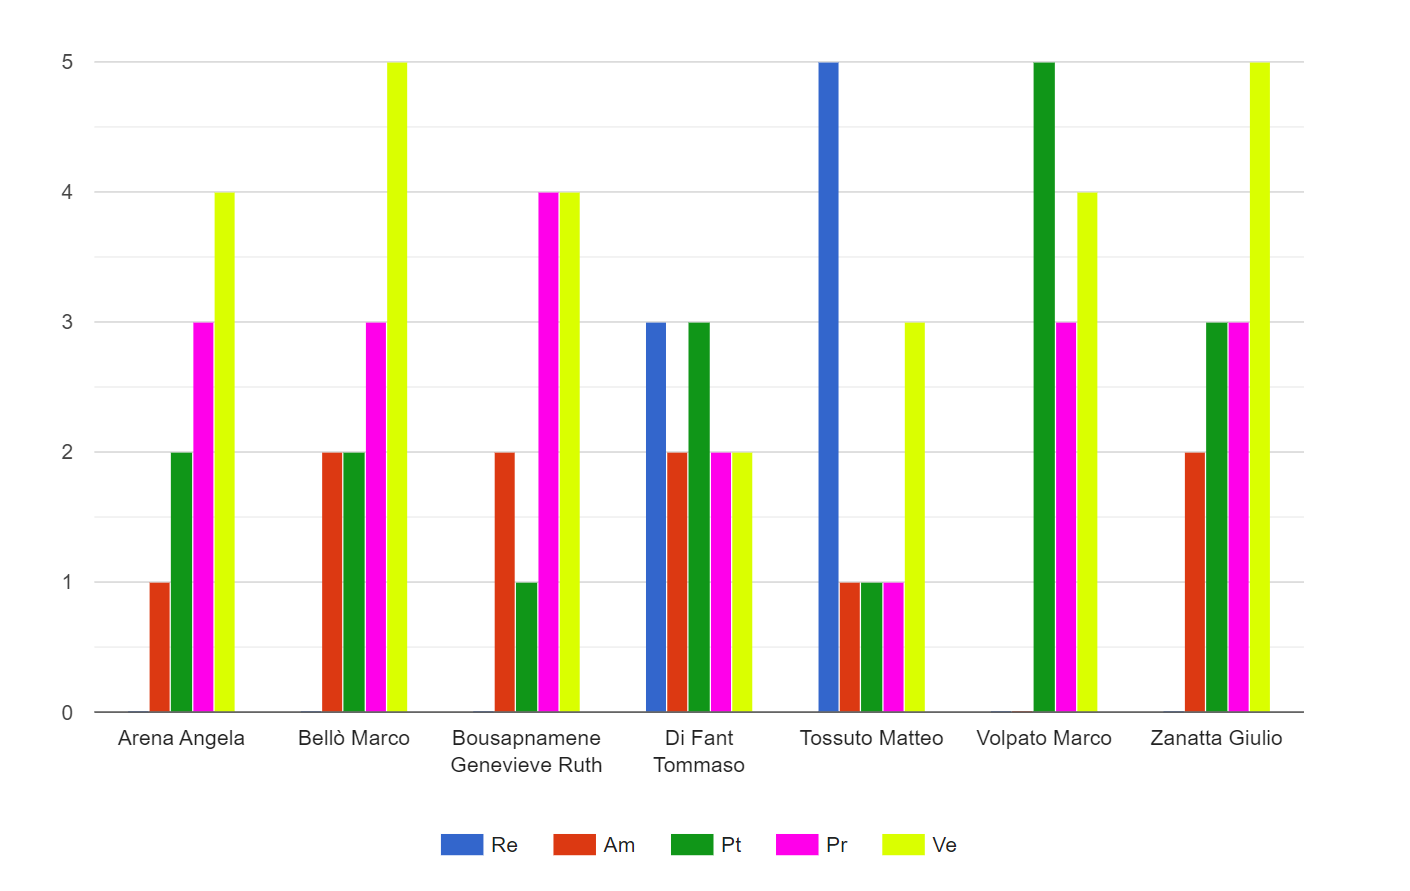
\includegraphics[width=15cm]{sezioni/Images/settimo.png}
        \centering
        \caption{Settimo incremento - Istogramma suddivisone ore per ruolo}
     \end{figure}
    }

    \subsubsection{Prospetto Economico}
    {
        \newcolumntype{L}[1]{>{\raggedright\let\newline\\\arraybackslash\hspace{1pt}}m{#1}}
        \newcolumntype{C}[1]{>{\centering\let\newline\\\arraybackslash\hspace{1pt}}m{#1}}
        \newcolumntype{R}[1]{>{\raggedleft\let\newline\\\arraybackslash\hspace{1pt}}m{#1}}
  
        \setlength{\freewidth}{\dimexpr\textwidth-30\tabcolsep}
        \renewcommand{\arraystretch}{1.0}
        \centering
        \setlength{\aboverulesep}{0pt}
        \setlength{\belowrulesep}{0pt}
        \begin{longtable}{C{.4\freewidth} C{.2\freewidth} C{.2\freewidth} C{.2\freewidth} C{.2\freewidth} C{.2\freewidth} C{.2\freewidth} C{.2\freewidth} C{.2\freewidth}}
          \toprule
        \rowcolor{Arancione}
        \textcolor{white}{\textbf{Ruolo}}&
        \textcolor{white}{\textbf{Ore}}&
        \textcolor{white}{\textbf{Costo}}\\
        \toprule
        \endhead
            
        Responsabile  & 8 & €240\\
        Amministratore  & 10 & €200 \\
        Analista &- & -\\
        Progettista &18 &€450\\
        Programmatore &20 & €300\\
        Verificatore &27 &€405\\
        Totale&84&€1595\\
        \\
        \caption{Settimo incremento - Costo per ruolo} 

        \end{longtable}

        \begin{figure}[H]
          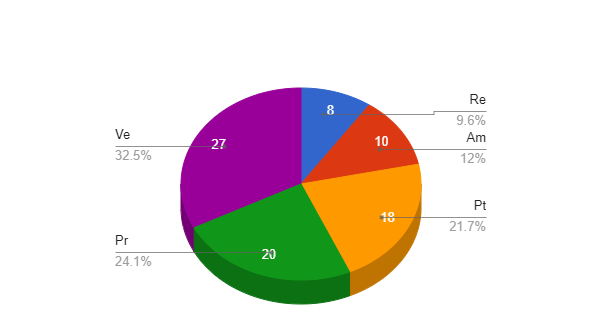
\includegraphics[width=15cm]{sezioni/Images/settimoT.png}
          \centering
          \caption{Settimo incremento - Grafico a torta costo per ruolo}
       \end{figure}
    }
    }

    \subsection{Ottavo incremento} 
    {
    \subsubsection{Prospetto orario}
    {
    Il gruppo per il ottavo incremento si impegna a rispettare tale ruoli come riportato in tabella:
    
    \newcolumntype{L}[1]{>{\raggedright\let\newline\\\arraybackslash\hspace{1pt}}m{#1}}
      \newcolumntype{C}[1]{>{\centering\let\newline\\\arraybackslash\hspace{1pt}}m{#1}}
      \newcolumntype{R}[1]{>{\raggedleft\let\newline\\\arraybackslash\hspace{1pt}}m{#1}}

      
      \setlength{\freewidth}{\dimexpr\textwidth-30\tabcolsep}
      \renewcommand{\arraystretch}{1.0}
      \centering
      \setlength{\aboverulesep}{0pt}
      \setlength{\belowrulesep}{0pt}
      \begin{longtable}{C{.4\freewidth} C{.1\freewidth} C{.1\freewidth} C{.1\freewidth} C{.1\freewidth} C{.1\freewidth} C{.1\freewidth} C{.1\freewidth} C{.1\freewidth}}
      \toprule
      \rowcolor{Arancione}
      \textcolor{white}{\textbf{Componente}}&
      \textcolor{white}{\textbf{Re}}&
      \textcolor{white}{\textbf{Am}}&
      \textcolor{white}{\textbf{An}}&
      \textcolor{white}{\textbf{Pt}}&
      \textcolor{white}{\textbf{Pr}}&
      \textcolor{white}{\textbf{Ve}}&
      \textcolor{white}{\textbf{Ore}}\\
      \toprule
      \endhead

      Arena Angela & - & 1 & -  & - & 1 & 5 & 7 \\
      \bottomrule
      Bellò Marco & - & 2 & - & - & 1 & 4 & 7 \\
      \bottomrule
      Bousapnamene & - & 1 & - & - & 1 & 4 & 6 \\
      \bottomrule
      Di Fant Tommaso & - & - & - & - & 1 & 5 & 6 \\
      \bottomrule
      Tossuto Matteo & - & 2 & - & - & 1 & 4 & 7 \\
      \bottomrule
      Volpato Marco & - & 2 & - & - & 1 & 3 & 6 \\
      \bottomrule
      Zanatta Giulio & 3 & - & - & - & 1 & 3 & 7 \\
      \bottomrule
      Totali & 3 & 8 & - & - & 7 & 28 & 46 \\
      \\
      \caption{Ottavo incremento - Suddivisione ore per ruolo}

      \end{longtable} 

      \begin{figure}[H]
        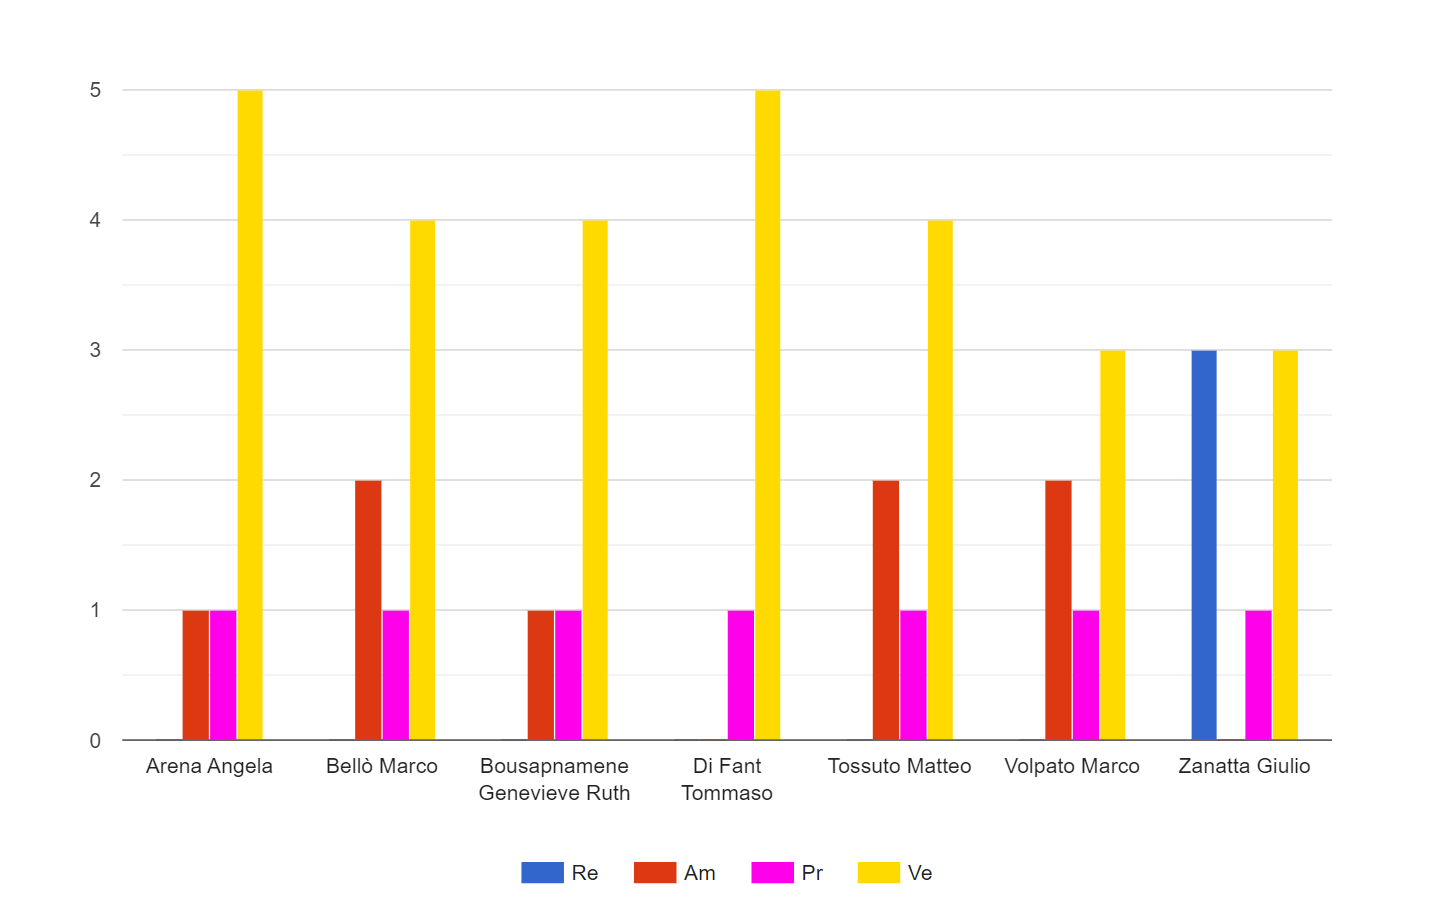
\includegraphics[width=15cm]{sezioni/Images/ottavo.png}
        \centering
        \caption{Ottavo incremento - Istogramma suddivisione ore per ruolo}
     \end{figure}
    }

    \subsubsection{Prospetto Economico}
    {
        \newcolumntype{L}[1]{>{\raggedright\let\newline\\\arraybackslash\hspace{1pt}}m{#1}}
        \newcolumntype{C}[1]{>{\centering\let\newline\\\arraybackslash\hspace{1pt}}m{#1}}
        \newcolumntype{R}[1]{>{\raggedleft\let\newline\\\arraybackslash\hspace{1pt}}m{#1}}
  
        \setlength{\freewidth}{\dimexpr\textwidth-30\tabcolsep}
        \renewcommand{\arraystretch}{1.0}
        \centering
        \setlength{\aboverulesep}{0pt}
        \setlength{\belowrulesep}{0pt}
        \begin{longtable}{C{.4\freewidth} C{.2\freewidth} C{.2\freewidth} C{.2\freewidth} C{.2\freewidth} C{.2\freewidth} C{.2\freewidth} C{.2\freewidth} C{.2\freewidth}}
          \toprule
        \rowcolor{Arancione}
        \textcolor{white}{\textbf{Ruolo}}&
        \textcolor{white}{\textbf{Ore}}&
        \textcolor{white}{\textbf{Costo}}\\
        \toprule
        \endhead
            
        Responsabile  & 3 & €90\\
        Amministratore  & 8 & €160 \\
        Analista &- & -\\
        Progettista &- &-\\
        Programmatore &7 & €105\\
        Verificatore &28 &€420\\
        Totale&46&€775\\
        \\
        \caption{Ottavo incremento - Costo per ruolo}
        \end{longtable}

        \begin{figure}[H]
          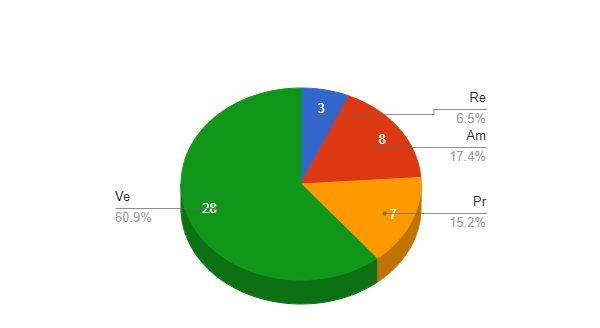
\includegraphics[width=15cm]{sezioni/Images/ottavoT.png}
          \centering
          \caption{Ottavo incremento - Grafico a torta costo per ruolo}
       \end{figure}
    }

    }


